\documentclass[a4paper]{article}
\let\subsubsubsection\paragraph
\let\subsubsubsubsection\subparagraph
\setcounter{secnumdepth}{4}
\setcounter{tocdepth}{4}
\usepackage[utf8]{inputenc}
%\usepackage[T1]{fontenc}
\usepackage[italian]{babel}
\usepackage{graphicx}
\usepackage{lscape}
\usepackage{fancyhdr}
\usepackage{totpages}
\usepackage{enumerate}
\usepackage{float}
\usepackage{color}
\usepackage[pdftex]{hyperref}
\usepackage{listings} 
\usepackage{tabularx}
\usepackage{amsthm}
\usepackage{amsmath}
\usepackage{listings}
\usepackage{mathtools}
\hypersetup{colorlinks,breaklinks,linkcolor=blue,urlcolor=black}

\usepackage[nolist]{acronym}
 
%%%%%%%%%%%%%%%%%%%%%% ACRONIMI %%%%%%%%%%%%%%%%%%%%%%
\begin{acronym}
    \acro{DSA}{Distributed Systems Annex}
    \acro{AWS}{Ada Web Server}
    \acro{FIFO}{first in first out}
    \acro{IDM}{Intelligent-Driver Model}
\end{acronym}

\usepackage[numbers,square,sort&compress]{natbib} 
\usepackage{fancyhdr}

\graphicspath{{img/}} 

\newcommand{\fncyblank}{\fancyhf{}}

\lstnewenvironment{codiceada}[1][] 
{\noindent\minipage{\linewidth}\medskip
\lstset{basicstyle=\footnotesize, columns=fullflexible,
keywordstyle=\color{red}\bfseries, commentstyle=\color{blue},
language=ADA, basicstyle=\small,
numbers=left, numberstyle=\small,
escapeinside={\%*}{*)},
extendedchars=false, captionpos=b,
title=\lstname, caption=\lstname,
stepnumber=1, numbersep=5pt, frame=single, #1}}{\endminipage}

%\newenvironment{abstract}%
%{\fncyblank\null\vfill\begin{center}%
%\bfseries\abstractname\end{center}}%
%{\vfill\null}

\renewcommand{\baselinestretch}{1.25}

%% per commenti vari

\usepackage{fixme} % remove draft option for final paper
\fxsetup{layout=inline,theme=color}
\FXRegisterAuthor{mn}{amn}{\color{green}mn} % marco negro
\FXRegisterAuthor{mb}{amb}{\color{blue}mb} % marco baesso


\pagestyle{fancy} 

\makeindex

% Definizione di nuovi "tokens" (e valori che possono assumere)
\newtoks\titolo
\newtoks\sottotitolo
\newtoks\filename
\newtoks\data
\newtoks\versione
\newtoks\distribuzione

% Titolo documento + titolo a pie' pagina e data (tokens)
\titolo={Relazione sull'esercitazione finale di Sistemi Concorrenti e Distribuiti} 
%\sottotitolo={Progetto di Sistemi concorrenti e distribuiti} 
\data={14/04/2015}

% Informazioni documento (tokens)
\filename={relazioneSCD.pdf}
\versione={1.0}
\distribuzione={Prof. Vardanega Tullio \\
		     	& Baesso Marco \\
			    & Negro Marco
}

% Header (left, center, right)
\lhead{} 
\chead{}
\rhead{}
\renewcommand{\headrulewidth}{0.4pt}
% Footer (left, center, right)
\lfoot{} \cfoot{} \rfoot{\thepage/\pageref{TotPages}}
\renewcommand{\footrulewidth}{0.4pt}

% Inizio documento LaTeX
\begin{document} %produce il titolo a partire dai comandi \title, \author e \date

\begin{center}
\vspace*{1,0 cm}
\huge\textbf{\the\titolo} \\ %LARGE != large
\vspace{0,4 cm}
\large\the\data
\end{center}
\begin{center}
\vspace{1,75 cm}

% Sommario
\begin{abstract} 
\begin{center}
Analisi del progetto didattico di Sistemi Concorrenti e Distribuiti. Considerazioni sulle scelte adottate e confronto con la soluzione proposta in corso di colloquio.
\end{center}
\end{abstract}
\vspace{1,50 cm}

% Informazioni documento
\textbf{Informazioni documento} \\ \vspace{0.5cm}
\begin{tabular}{r | l }
\textbf{Nome file}      & \the\filename         \\
\textbf{Versione}       & \the\versione         \\
\textbf{Distribuzione}  & \the\distribuzione    \\ \\
\end{tabular}
\vspace{0,3cm}
\end{center}

\newpage

\tableofcontents


\newpage
\section{Introduzione}
Questo documento ha come scopo quello di fornire un'analisi delle scelte
progettuali dell'esercitazione svolta per il corso di Sistemi Concorrenti e
Distribuiti, che prevedeva lo studio e la prototipazione di un simulatore di
traffico viario in una città con requisiti funzionali a discrezione degli
esaminandi. Tale documento è strutturato definendo il problema e la soluzione
suggerita nel corso dei colloqui orali e nelle conversazioni avvenute via mail,
per procedere poi con l'analisi delle scelte progettuali di distribuzione e
concorrenza effettuate al fine di risolvere il problema proposto.

\section{Analisi del dominio del problema}
In questa sezione viene descritta la consegna data integrata con i nostri requisiti funzionali. La consegna iniziale prevedeva la realizzazione di una simulazione del traffico in una città. \\
L'obiettivo dell'analisi del dominio è quello di fissare dall'inizio quello che il simulatore deve fare in termini di funzionalità di cui l'attore dello spostamento deve essere dotato.

\subsection{Entità rappresentate nella mappa della città}
\label{firstmappa}
La mappa della città è caratterizzata da strade dotate di doppia corsia per senso di marcia, d'ora in poi \textit{\textbf{strade principali}}, (possono essere sostitute nel corso della relazione con il sinonimo di strade urbane), marciapiedi, piste ciclabili, \textit{\textbf{strade di ingresso}} al traffico, incroci, dotati di semaforo, con 3 o 4 strade e attraversamenti pedonali.\\
Sono stati identificati come attori del traffico della città simulata: veicoli (auto e autobus), biciclette e pedoni.

\subsection{Requisiti sullo spostamento delle entità}
\begin{enumerate}
\item {\textit{requisito relativo al mezzo di spostamento degli attori}}: deve essere data la possibilità di configurare il mezzo di spostamento dell'attore che verrà adottato poi per tutta la durata della simulazione;
\item {\textit{requisito relativo ai luoghi di destinazione degli attori}}: un attore deve poter essere configurato in modo tale da muoversi nella città al fine di spostarsi verso un certo luogo di destinazione.
Un attore quindi una volta raggiuta la destinazione dovrà reimmetersi nel traffico per raggiungere il luogo da cui era partito, iterando quindi l'avanzamento da luogo di partenza a luogo di destinazione e viceversa. L'obiettivo di questo requisito è quello di avere una situazione in cui nella città vi sia sempre del traffico nel caso in cui almeno un'entità sia presente.
\end{enumerate}

\subsection{Convenzioni sulla mappa}
A seguito dell'analisi è stato convenuto riportare delle regole sulla realizzazione della mappa avendo fissato a priori le entità sulle quali gli attori dovevano eseguire lo spostamento, vedi \ref{firstmappa}.
\begin{enumerate}
\item una strada principale deve essere delimitata almeno da un incrocio e al più da due incroci;
\item una strada di ingresso è una strada adibita all'entrata o all'uscita da o verso un certo luogo;
\item una strada principale presenta due lati ai quali possono essere inserite delle strade di ingresso; quindi se su una stessa strada principale vengono inserite più strade di ingresso è convenuto imporre che queste strade tengano una distanza minima l'una dall'altra, indipendentemente dal lato della strada principale in cui vengono inserire; l'obiettivo è quello di evitare che si formi un incrocio tra strade di ingresso non regolamentate da semaforo;
\item ogni strada principale contiene esattamente una fermata per l'autobus posta a seconda della configurazione della mappa su uno dei due lati della strada principale stessa.
\end{enumerate}

\subsection{Altri requisiti rilevati dall'analisi del dominio}
Nell'analisi del dominio del problema sono state identificate quindi le entità che sono rilevanti per la realizzazione del simulatore e sono state definite delle regole e quindi delle limitazioni funzionali per la realizzazione della mappa. \\
Sono emerse inoltre le seguenti funzionalità e requisiti a seguito di un'analisi a livello anche progettuale:
\begin{enumerate}
\item un entità del tipo veicolo che deve svoltare a sinistra al prossimo incrocio dovrà immettersi ad un certo punto nella corsia più a sinistra della strada che sta percorrendo; se il veicolo dovrà andare a destra dovrà immettersi nella corsia più a destra della strada che sta percorrendo e indifferentemente su entrambe le corsie se vuole procedere in direzione dritto;
\item un entità del tipo veicolo deve poter agevolmente cambiare corsia su una strada principale in modo tale da poter raggiungere la corsia interessata in relazione alla destinazione da perseguire;
\item il percorso che l'entità di tipo veicolo, bipede, o bici deve percorrere deve essere fissato a priori. \\
Questa è una limitazione per la simulazione, ma per semplicità anche di implementazione è stato convenuto definire un percorso statico piuttosto che dinamico;
\item un pedone o una bici non eseguono dei sorpassi, ma procedono secondo una politica FIFO nell'avanzamento rispettivamente nel marciapiede e nella pista ciclabile. 
\end{enumerate}

\newpage


\section{Strategie di distribuzione}
In questa sezione vengono esposte le scelte progettuali di distribuzione.

\subsection{Due possibili strategie di distribuzione}
\label{scelted}
Nella simulazione del traffico di una città, la politica di distribuzione che 
potrebbe ragionevolmente portare più benefici consiste nella segmentazione 
della dimensione della città. Questa politica, infatti, permette la distribuzione
su nodi diversi della simulazione dell'intera città. 
Seguendo questo approccio la città risulterebbe partizionata in quartieri, i
quali rappresenterebbero i frammenti dell'intera mappa della città, suddividendo
così su più nodi il luogo della realizzazione dello spostamento delle entità. 

Un'altra possibile strategia potrebbe essere quella di conservare in un unico
luogo la mappa, centralizzando su un singolo nodo lo stato di avanzamento del
sistema. Questa strategia non gode tuttavia della proprietà della scalabilità
della mappa: come si comporterebbe il sistema nel caso cambiasse la
configurazione della mappa e le dimensioni fossero notevoli? 
D'altro canto, questa strategia semplificherebbe di molto
la gestione dell'orologio virtuale per l'avanzamento delle entità del tipo veicolo,
bici o pedone dato che tutto, secondo la strategia in questione, diviene
centralizzato. Seguendo questa strategia la distribuzione potrebbe ricadere non
più sulla mappa ma sulle entità da spostare. Tuttavia il nodo che conserva
l'intera mappa diverrebbe un collo di bottiglia per gli aggiornamenti di stato
delle entità. 

\subsection{Strategia di distribuzione scelta}
La strategia scelta è la prima tra quelle esposte in \ref{scelted}. Questo
sistema risulta il più desiderabile in quanto sfrutta in modo adeguato il
concetto di distribuzione, permettendo così la gestione dei calcoli per
l'avanzamento delle entità e delle richieste su più nodi.

\subsection{Definizione dei ruoli delle entità del sistema}
Le entità esposte in \ref{firstmappa} meritano un ruolo in funzione della
strategia di distribuzione scelta. Fondamentalmente, le entità in un sistema
concorrente e distribuito vengono distinte in attive e reattive.
Assegnando il ruolo di entità attiva a veicoli, bici o pedoni si presenterebbe
un problema relativo al loro spostamento nel caso in cui essi debbano muoversi
da un quartiere all'altro.
Dato che le entità attive richiedono un processo, nel momento in cui un oggetto
debba spostarsi tra due quartieri, si incorrerebbe in un inutile spreco di
risorse, andando ad impattare anche le prestazioni del sistema.
Infatti, si avrebbe un processo inutile istanziato in un quartiere e
occorrerebbe istanziare uno di completamente nuovo nel quartiere di destinazione
dell'entità.
Questo potrebbe essere un problema dato che vengono istanziati dinamicamente dei
processi: si potrebbero ottenere errori a run-time nel caso in cui il nodo non
riesca ad istanziare il nuovo task.

L'alternativa potrebbe essere preallocare un certo numero di thread per ospitare
le entità che richiedono di essere spostate nel quartiere interessato.
A questo punto, però, occorrerebbe porre una limitazione sul numero di entità
che un certo quartiere potrebbe ospitare.
Questo risulterebbe quindi poco scalabile e scomodo da gestire nel caso in
cui un'entità attiva debba rimanere in attesa che il quartiere di
destinazione liberi un thread, dal proprio thread-pool di risorse preallocate,
per poterla eseguire.

Il ruolo di entità attiva dovrebbe ricadere quindi sugli oggetti di tipo strada
o incrocio. 
Dato che la mappa presenta, una volta configurata e istanziata, una un numero
costante di elementi, si avrà che il sistema non necessiterà di istenziare
dinamicamente dei processi.
Inoltre, ogni partizione per soddisfare le richieste di altre partizioni se
dotata di un thread-pool risolve anche il problema dell'allocazione di thread
per richieste remote da soddisfare.

Seguendo questa strategia il sistema diviene scalabile sia in termini di
distribuzione che di concorrenza.

\subsection{Componenti oggetto della distribuzione}\label{subsec:distribuzione}
\begin{figure}[H] % Example image
\center{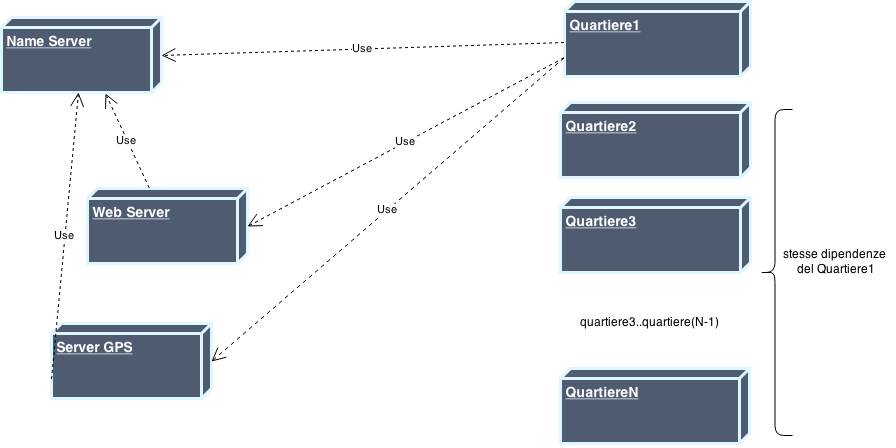
\includegraphics[width=1.0\linewidth]{DiagrammaComponenti}}
\caption{Diagramma componenti.}
\label{fig:Diagramma componenti}
\end{figure}
In questa sezione vengono descritte le componenti del sistema:
\begin{description}
\item[Quartiere:] componente che deve essere istanziata per ogni frammento della
mappa previsto dalla configurazione. Se un quartiere presenta una configurazione
valida, esso può entrare a far parte del sistema in qualunque momento (entro il
limite previsto del numero massimo di quartieri istanziabili).
Un quartiere è responsabile dello spostamento delle entità che sono in transito
in una qualunque delle strade o incroci che appartengono al quartiere stesso. Le
entità reattive quali i veicoli, le bici e i pedoni vengono istanziate in uno
specifico quartiere e le informazioni relative allo stato del percorso di queste
entità saranno sempre reperibili dal quartiere al quale l'entità è stata
istanziata, al fine di evitare che nel momento in cui un'entità debba essere
spostata da un quartiere all'altro, non occorra riportare tutto lo stato del
percorso al quartiere interessato.

Dato che, una volta configurato il sistema, le entità reattive non cambiano in
numero e contenuto informativo, conviene riportare per ogni quartiere una cache
delle entità di ogni altro quartiere al fine di evitare un numero eccessivo di
richieste a quartieri remoti responsabili dell'istanziazione delle entità
interessate durante le fase di avanzamento delle entità.
\item[Server GPS:] è una componente passiva che si occupa del calcolo del
percorso per conto di una entità. Questa componente dispone della conoscenza
della mappa di ogni quartiere correttamente istanziato. Il server GPS effettua
un aggiornamento della mappa in relazione alle nuove richieste di istanziazione
di nuovi quartieri. Il calcolo del percorso avviene eseguendo l'algoritmo di
Dijkstra dei cammini minimi. Se una certa entità deve muoversi verso una certa
destinazione non ancora raggiungibile, a causa del fatto che il quartiere
interessato non è stato ancora istanziato occorrerà ritardare lo spostamento
dell'entità. Il server per una stessa entità potrebbe calcolare percorsi minimi
diversi per 2 richieste diverse nel caso in cui nel frattempo è stato istanziato
un nuovo quartiere che presenta un percorso più breve per raggiungere la
destinazione.
\item[Web Server:] è la componente responsabile della creazione della view e
del rendering dello stato di avanzamento delle entità del sistema.
\item[Name Server:] si occupa invece di servire alle altre partizioni richieste
di accesso e riferimento a risorse che risiedono su una partizione remota.
\end{description}
\section{Strategia di avanzamento delle entità di tipo veicolo, bici o pedone}
Un primo approccio per l'avanzamento delle entità passive (veicoli, bici,
pedoni) era quello di suddividere la strada in segmenti di breve lunghezza e
permettere l'attraversamento di uno speyyone di strada ad una sola entità per
volta.
Questa strategia porta ad un avanzamento per distanze di sicurezza, ma
l'aggiornamento della nuova posizione avrebbe portato ad un avanzamento ``a
scatti'' del sistema, al di la di eventuali ottimizzazioni.

Quello che in realtà occorre considerare nell'avanzamento delle entità sono le
proprietà intrinseche del moto di avanzamento, ovvero il tempo, lo spazio,
l'accelerazione e la decelerazione. La strategia scelta segue una logica di
avanzamento secondo il modello \ac{IDM}~\cite{treiber2000microscopic}.
Seguendo il modello \ac{IDM}, l'avanzamento avviene considerando il
\textbf{\textit{delta}} di tempo nel quale il mezzo deve avanzare e le proprietà
del veicolo stesso. In relazione a questi parametri viene calcolata una
percentuale sull'accelerazione massima con cui il mezzo è stato configurato.
Infine, utilizzando il valore dell'accelerazione ottenuto, viene aggiornata la
velocità corrente e la posizione finale del mezzo.
Questi nuovi valori saranno validi alla fine del delta di tempo relativo al
periodo in cui sono stati calcolati. Di seguito vengono riportate le funzioni
matematiche utilizzate per il calcolo dello spostamento delle entità:

\begin{equation}
s^{*}(t)=s(0)+Tv(t)+\frac{v(t)\Delta{v(t)}}{2\sqrt{ab}}
\end{equation}
\begin{equation}
a(t)=a[1-(\frac{v(t)}{v_{0}})^4-(\frac{s^{*}(t)}{s(t)})^2]
\end{equation}
dove
\begin{align*}
~a =&~\text{massima accelerazione possibile}\\
v_{0} =&~ \text{elocità desiderata} \\
v(t) =&~ \text{velocità corrente} \\
s(t) =&~ \text{distanza corrente dal mezzo che sta davanti} \\
s_{0} =&~ \text{quantità minima di avanzamento} \\
s^*(t) =&~ \text{distanza calcolata in funzione dei parametri di configurazione}
\\ &~ \text{dei mezzi interessati} \\
T =&~ \text{parametro di controllo per regolamentare la velocità} \\
b =&~ \text{decelerazione massima}
\end{align*}

% $a$ è la massima accelerazione possibile; $v_{0}$ è la velocità desiderata;
% $v(t)$ è la velocità corrente; $s(t)$ è la distanza corrente dal mezzo che sta
% davanti; $s_{0}$ è la quantità minima di avanzamento; $s^*(t)$ è la distanza
% calcolata in funzione dei parametri di configurazione dei mezzi interessati; $T$
% è un altro parametro di controllo per regolamentare la velocità; $b$ è la
% decelerazione massima.

Infine è possibile aggiornare la velocità corrente della macchina e lo step di
avanzamento($ns(t)$): 

\begin{equation}
v(t)= v(t)+a\Delta
\end{equation}
\begin{equation}
ns(t)= v(t)\Delta+0.5a\Delta^2
\end{equation}

con $\Delta$ uguale al tempo desiderato per calcolare la posizione del mezzo
alla fine del $\Delta$ stesso. 

Il modello permette quindi di rappresentare una realtà continua relativa
all'avanzamento delle entità, discretizzando il tempo per una quantità $\Delta$.
In pratica, viene dato in input al modello \ac{IDM} lo stato del mezzo,
contenente la posizione corrente e i parametri di avanzamento.
Il modello ritornerà dei valori relativi all'aggiornamento della posizione delle
entità, i quali saranno validi per il modello a realtà continua alla fine
del $\Delta$ di tempo relativo al periodo in cui sono stati calcolati.

Il modello presentato richiede quindi una configurazione di alcuni parametri,
tra i quali le proprietà di moto delle entità e un parametro di sistema, ovvero
il $\Delta$. La configurazione dei parametri delle entità può essere lasciata
all'utente, predisponendo dei valori di default al fine di accelerare il
processo di configurazione delle entità.

Si è convenutio di assegnare a $\Delta$ un valore costante, quindi non
configurabile dall'utente. La scelta di tale quantità, ovvero la durata
del quanto di discretizzazione deve seguire la seguente logica:
se il $\Delta$ viene tarato con valori grandi (nell'ordine dei secondi) allora
il sistema eseguirebbe meno calcoli per completare gli spostamenti delle entità.
D'altro canto, al crescere del $\Delta$ la simulazione risulterebbe rallentata
dal punto di vista dell'avvenimento di alcuni eventi dovuti per conseguenza di
altri, ovvero le entità sarebbero poco reattive e ritarderebbero le loro azioni
in funzione della grandezza del $\Delta$. Se il $\Delta$ è troppo piccolo
(nell'ordine dei millisecondi) il sistema si troverebbe nella situazione di
eseguire molti calcoli per completare lo spostamento, le entità sarebbero
reattive, ma la quantità di avanzamento effettiva di una entità sarebbe minuta e
inutile al fine della reattività instantanea delle altre entità presenti nel
sistema. Il valore del $\Delta$ da noi scelto è \textbf{\textit{0.5 secondi}},
cosi da permettere il giusto compresso tra step di avanzamento delle entità e
reattività delle entità.
\section{Gestione del tempo tra quartieri}
Il problema principale della frammentazione della mappa in quartieri consiste nella gestione del $\Delta$ di avanzamento tra quartieri; i quartieri non possono avanzare indipendentemente l'uno dall'altro; cioè un quartiere che ha effettuato i calcoli per l'avanzamento per un certo $\Delta$, non può procedere a effettuare il calcolo di nuovi spostamenti per un nuovo $\Delta$ fino a quando tutti gli altri quartieri non hanno completato l'aggiornamento degli spostamenti delle entità al $\Delta$ precedente. Lo spostamento delle entità dei quartieri deve essere trasparente alla distribuzione della mappa, quindi un quartiere presenta una dipendenza dagli altri quartieri affinchè tutti i quartieri siano sincronizzati allo stesso quanto di tempo discretizzato. Ancora più evidente è il caso in cui un quartiere presenta un incrocio in cui per esempio una delle sue strade appartenga ad un altro quartiere; se il sistema non è sincronizzato allo stesso quanto di tempo si potrebbe incorrere nella situazione in cui un certo mezzo che debba essere spostato tra due quartieri, si trovi in attesa che il quartiere di destinazione si risincronizzi al quanto successivo; quindi avere una situazione in cui l'entità si trovi in attesa indipendentemente dalla velocità e dallo stato del traffico.\\
Dato che le entità attive del sistema sono le strade e gli incroci e la responsabilità dell'esecuzione del calcolo dell'avanzamento in un certo quanto di tempo è data sempre alle entità attive, queste dovranno rendersi partecipi nel regolamentare l'avanzamento del sistema al quanto di tempo successivo.\\

\subsection{Protocollo di sincronizzazione}
Questo protocollo si occupa di regolamentare l'avanzamento del sistema al quanto di tempo successivo; questo protocollo è quindi responsabile della gestione della logica di discretizzazione del tempo per permettere di avere una realtà continua consistente in ogni quartiere.\\
Per lo sviluppo di questo protocollo occorre considerare dapprima come il sistema viene avviato; cioè se il sistema attende che tutti i quartieri siano configurati e quindi tutti i quartieri partiranno in sincronia al tempo 0; oppure se si sceglie un approccio più flessibile in cui un quartiere viene configurato indipendentemente dagli altri e quindi entrerà in sincronizzazione in un momento non necessariamente corrispondente al tempo 0. Occorre considerare che un quartiere è una partizione a se stante, che presenta tuttavia delle dipendenze con gli altri quartieri; entrambi i sistemi di avvio presentano dei vantaggi: nel primo caso si ha che ogni quartiere aspetta che gli altri si siano configurati, si avrà quindi un ritardo nell'avvio, ma quando un quartiere ritorna dall'attesa può reperire ogni risorsa di qualunque altro quartiere dato che al ritorno dall'attesa il tutto è stato configurato; tuttavia seguendo questa idea si potrebbe presentare il caso in cui si potrebbero avere dei quartieri isolati che aspettano inutilmente altri quartieri o comunque si renderebbe impossibile la possibilità di voler aggiungere in seguito all'avvio della simulazione altri quartieri.\\
Il secondo caso invece è quello che si avvicina di più a ciò che è il paradigma della distribuzione, lasciando quindi l'indipendenza nella fase di avvio tra quartieri e quindi permettendo comunque lo spostamento di tutte le entità che presentano un percorso valido relativo al quartiere stesso, mentre per le entità che presentano delle destinazioni non raggiungibili il quartiere ne dovrà ritardare lo spostamento. Il nostro sistema implementa questa seconda scelta lasciando ove possibile l'indipendenza tra le partizioni, permettendo l'avvio del sistema e quindi dello spostamento delle entità indipendentemente dal fatto che una partizione remota sia stata configurata o meno.\\
Solo quando un quartiere presenterà richiesta di sincronizzazione allora il sistema dovrà tener conto anche della sua richiesta per permettere l'avanzamento al quanto di tempo successivo in modo da coinvolgere ogni quartiere che necessita di essere sincronizzato.\\
Tuttavia se un quartiere è stato istanziato e ha iniziato l'operazione di sincronizzazione con gli altri quartieri, in caso di fallimento o di errore durante l'esecuzione di uno qualunque di questi quartieri sincronizzati il sistema non potrà che fermarsi dato che un quartiere esegue dei servizi di spostamento per conto di entità di altri quartieri; se un quartiere da errore durante l'esecuzione lo stato del sistema diviene inconsistente e occorre riavviare il sistema e se necessario farlo ripartire dall'ultima snapshot del sistema una volta istanziati tutti i quartieri che erano stati avviati e sincronizzati all'ultima snapshot disponibile.\\
Il protocollo di sincronizzazione dovrà quindi considerare la possibilità di accogliere dei nuovi quartieri da rendere parteci alla sincronizzazione.\\
Il protocollo di sincronizzazione si divide in due parti: la sincronizzazione tra entità attive del quartiere (\ref{int_synch}) e la sincronizzazione tra quartieri (\ref{quart_synch}).
\subsubsection{Sincronizzazione tra entità attive del quartiere}
\label{int_synch}
Ogni entità attiva del quartiere dovrà comunicare ad un gestore della sincronizzazione interna del quartiere, che ha eseguito l'aggiornamento dello stato di avanzamento delle entità passive per un certo $\Delta$ di sistema. L'entità attiva dovrà poi attendere che tutto il sistema sia sincronizzato con il $\Delta$ di sistema. Solo quando l'ultima entità attiva del quartiere in questione ha eseguito l'avanzamento al $\Delta$ di sistema allora questa entità potrà avviare il protocollo di sincronizzazione tra quartieri, vedi \ref{quart_synch}.

\subsubsection{Sincronizzazione tra quartieri}
\label{quart_synch}
Il seguente protocollo è un protocollo che esegue la sincronizzazione tra un numero di quartieri non fissato a priori. Di seguito i passi del protocollo (ogni volta che appare il nome di quartiere si intenderà l'entità responsabile della sincronizzazione di tutti i quartieri allocata nel quartiere stesso):
\begin{enumerate}
\item il quartiere deve ottenere dapprima dal name server il registro dei quartieri remoti che abbiano effettuato la registrazione della mappa al server gps (da notare che quartieri distinti potrebbero ricevere risposte diverse dal nameserver, ma risposte successive saranno sempre al più un sovrainsieme delle risposte date in precedenza);
\item il quartiere (Q\_X) per ogni quartiere presente nel registro dovrà inviare una notifica testimone del fatto che Q\_X è pronto per una nuova sincronizzazione. Tale notifica potrà essere gestita dal quartiere interessato (Q\_Y) solo nel momento in cui anche Q\_Y è pronto per una nuova sincronizzazione, ovvero quando inizierà a eseguire anch'esso il protocollo (\ref{quart_synch}). L'esecuzione della procedura di notifica su Q\_Y andrà a buon fine nel caso in cui Q\_Y dispone nel proprio registro del quartiere Q\_X e in tal caso occorrerà salvare su Q\_Y il fatto che Q\_X è pronto per una nuova sincronizzazione; altrimenti Q\_Y accoda la notifica di Q\_X (lasciando in stato di attesa quindi la partizione Q\_X) al fine di poterla gestire nel quanto successivo in cui a quel punto Q\_Y certamente otterrà dal name server anche Q\_X nello step 1 del protocollo. \\
Ogni quartiere ha degli eventi che permettono di decidere il momento in cui esso può eseguire le notifiche di richiesta di nuova sincronizzazione. L'evento che permette di eseguire le procedure di notifica su Q\_Y richieste da quartieri remoti Q\_X è il passaggio dall'esecuzione di \ref{int_synch} a \ref{quart_synch} e in particolare l'esecuzione dello step 1 del protocollo. \\ La disabilitazione dell'esecuzione della procedura di notifica, operazione di \textit{CLOSE\_SYNCH}, su Q\_Y deve avvenire dall'ultimo quartiere utile che esegue su Q\_Y la procedura di notifica. Dove per ultimo quartiere utile si intende quell'ultimo quartiere (indipendentemente dall'ordine) che appartiene all'insieme minimo dei quartieri tra tutti gli insiemi di quartieri presenti nei registri dei quartieri stessi presi nello step 1 del protocollo (tale insieme d'ora in poi verrà chiamato \textit{MIN\_SET\_QUARTIERI}). \\
\item ogni quartiere presente in \textit{MIN\_SET\_QUARTIERI} dovrà quindi aspettare l'evento di chiusura della gestione delle notifiche di nuova sincronizzazione, ovvero l'evento \textit{CLOSE\_SYNCH}; a questo punto un quartiere uscente dall'attesa non conosce più lo stato di avanzamento degli altri quartieri, cioè è solo a conoscenza del fatto che tutti i quartieri in \textit{MIN\_SET\_QUARTIERI} hanno presentato nuova richiesta di sincronizzazione, ma nel frattempo uno dei quartieri in \textit{MIN\_SET\_QUARTIERI} potrebbe aver iniziato nuovamente ad eseguire il protocollo sovrascrivendo l'esecuzione delle notifiche e quindi perdendo una notifica di nuova sincronizzazione da parte di un quartiere se l'evento \textit{CLOSE\_SYNCH} non era ancora giunto. Pertanto è necessario che ogni quartiere, prima di poter eseguire nuovamente una nuova sincronizzazione, attenda l'evento \textit{CLOSE\_SYNCH} che sarà inviato da ogni altro quartiere presente in \textit{MIN\_SET\_QUARTIERI};
\end{enumerate}
Tra lo step 1 e 2 occorre integrare il seguente punto:  
\begin{itemize}
\item il quartiere deve liberare dall'attesa, se presenti, tutti quei quartieri che al $\Delta$ di sincronizzazione precedente non erano nel registro dei quartieri, supponiamo che Q\_Y nel proprio registro non contenga Q\_X, mentre Q\_X contiene nel proprio registro Q\_Y; mentre il quartiere remoto Q\_X si presta in attesa sul quartiere Q\_Y, Q\_Y non considerà Q\_X. Quindi Q\_X deve essere classificato come un quartiere nuovo che potrà entrare in sincronizzazione solo al $\Delta$ successivo; tuttavia Q\_X potrebbe nel frattempo già aver demandado l'esecuzione dello step 2 su altri quartieri che contenevano nel proprio registro Q\_X; ebbene questi quartieri dovranno ricordare tale fatto nel loro $\Delta$ di sincronizzazione successivo, dato che Q\_X a questi quartieri non invierà più la notifica di sincronizzazione; mentre Q\_Y dovrà accodare Q\_X fino alla richiesta di sincronizzazione successiva in cui appunto verrà riaccodato dallo step appena descritto nella procedura di gestione delle notifiche per il nuovo $\Delta$.
\end{itemize}

\begin{figure}[H] % Example image
\center{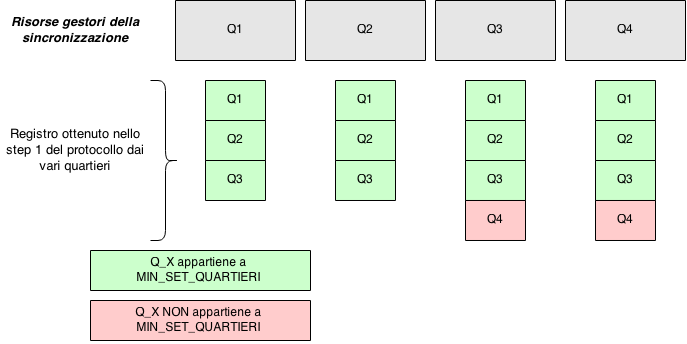
\includegraphics[width=1.0\linewidth]{ProtocolloSynch}}
\caption{Esempio di stato nella sincronizzazione dei quartieri.}
\label{fig:Esempio di stato nella sincronizzazione dei quartieri}
\end{figure}

Nell'esempio riportato i quartieri soggetti a sincronizzazione saranno Q1,Q2,Q3 mentre Q4 non potrà partecipare alla sincronizzazione, se non prima della sincronizzazione successiva in cui certamente Q1 e Q2 alla nuova richiesta del registro al name server otterranno anche Q4. Q4 cosa può fare dato che non può partecipare alla sincronizzazione? Esso potrebbe presentare una richiesta a Q1 o Q2 e in tal caso rimmarrebbe bloccato sul quartiere Q1 o Q2 dato che entrambi non dispongono di Q4; Q4 potrebbe anche presentare la richiesta a Q3 e in tal caso Q3 accoglierà Q4 e salverà temporaneamente una flag che lo avviserà per il prossimo quanto che Q4 ha già presentato richiesta di sincronizzazione. Q3 sa inoltre che non potrà attendere Q4 dato che nel momento in cui Q1 o Q2 presenteranno richiesta di sincronizzazione a Q3 invieranno anche il loro registro e li Q3 apprenderà che Q4 non è un quartiere sul quale occorre aspettare e quindi non è rilevante all'evento \textit{CLOSE\_SYNCH} nel corso del $\Delta$ corrente. Con questo semplice esempio è stato presentato un caso di sincronizzazione; ma ce ne possono essere di più complicati per esempio nel caso in cui esistesse anche un quartiere Q5 non visibile a nessuno. In tal caso alla nuova sincronizzazione Q1 Q2 e Q3 memorizzeranno nel loro registro anche Q5, mentre per Q4 il quartiere Q5 sarà un quartiere nuovo e quindi quest'ultimo potrà entrare in sincronizzazione solo al quanto successivo.

\paragraph{Considerazioni sul protocollo \ref{quart_synch}}
Questo protocollo si adatta dinamicamente a nuove richieste di sincronizzazione. Il difetto principale sta nel fatto che un quartiere dovrà attendere su altri quartieri al fine di apprendere se tutto il sistema è pronto per il passaggio al quanto successivo. In realtà l'attesa potrebbe essere rigirata sul quartiere stesso e non più sul quartiere remoto, ma data la limitazione sul numero massimo di quartieri non è un problema l'implementazione di questo protocollo anche se i quartieri utilizzano un thread-pool nella gestione delle richieste remote.
\section{Protocollo per l'istanziazione di una partizione di tipo quartiere}
La partizione può iniziare ad operare solo dopo che le componenti di name server e server gps sono state correttamente istanziate; la componente dovrà poi eseguire le seguenti operazioni:
\begin{enumerate}
\item deve essere configurata la mappa del quartiere, in relazione al file di configurazione dato in input alla componente, e quindi occorre creare tutte le entità attive che la partizione vede partecipe (strade, incroci), tutte le entità passive (veicoli, bici e pedoni), e tutte quelle risorse che possono essere riferite da una partizione remota (gestore delle risorse di tipo autobus, gestore del servizio di locazione delle entità passive, risorsa utilizzata per ottenere informazioni sul quartiere, risorse in gestione alle entità attive per memorizzare lo stato di avanzamento delle entità passive);
\item il quartiere deve poi procedere a registrare al name server le risorse riferibili da remoto; tale operazione deve essere un'operazione atomica che può o meno andare a buon fine, per esempio essa sarà rifiutata se un quartiere con lo stesso identificativo è già stato registrato;
\item se l'operazione precedente è avvenuta con successo, la componente del quartiere dovrà procedere con la registrazione della configurazione della mappa al server gps e quindi a operazione terminata dovrà comunicare al name server che il quartiere in questione ha correttamente configurato la propria mappa nel server gps; a questo punto il quartiere sarà un quartiere correttamente istanziato ed ogni altro quartiere avrà la visibilità del quartiere appena creato; fintanto che il quartiere non ha registrato la sua presenza al name server, eventuali operazioni di errore nella partizione non sono compromettenti per la consistenza dello stato dell'intero sistema, mentre se il quartiere ha eseguito la propria registrazione nel name server allora ogni errore che avverrà durante l'esecuzione di tale partizione genera uno stato inconsistente per il sistema e sarà necessario quindi eseguire un'operazione di riavvio; 
\item se la partizione si trova in stato di errore dovrà terminare, altrimenti può procedere con l'esecuzione del protocollo di sincronizzazione, vedi \ref{protosynch}.
\end{enumerate}
\newpage
\section{Protocolli tra entità attive del sistema}
Seguendo il modello IDM un parametro importante da considerare per l'avanzamento delle entità passive è la distanza tra l'entità stessa e la fine della traiettoria del mezzo che si trova davanti o che l'entità potrebbe trovarsi davanti a seguito di uscite da ingressi o cambi corsia di altri mezzi che si trovano davanti al mezzo interessato. Tutta la logica dell'avanzamento viene quindi basata sul calcolo delle distanze ai mezzi antecedenti il mezzo interessato. Il calcolo di questa distanza deve essere fatto in relazione alla posizione del mezzo che copriva nel quanto di tempo antecedente al quanto di tempo in cui viene effettuato l'aggiornamento della nuova posizione (anche per questo motivo il $\Delta$ del sistema non può assumere valori troppo grandi). Ribadendo quali sono le entità attive del sistema: incroci, strade principali, strade d'ingresso è necessario stabilire dei protocolli di comunicazione tra le entità. In particolare conviene dapprima fissare un ordine di esecuzione per le entità attive:

\begin{figure}[H] % Example image
\center{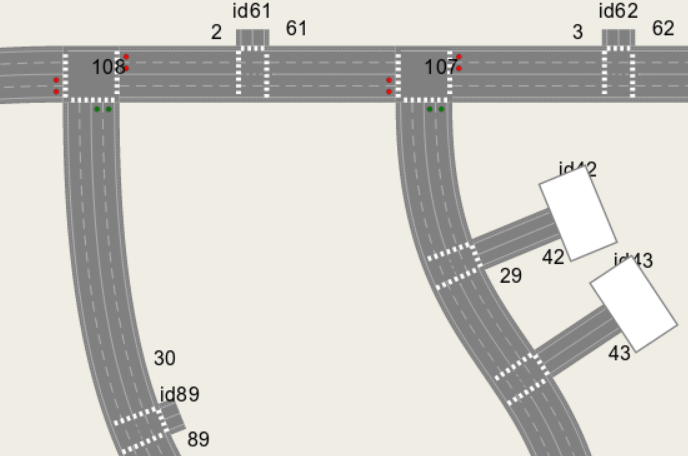
\includegraphics[width=0.9\linewidth]{EsempioMappa}}
\caption{Un frammento di mappa di un quartiere.}
\label{fig:Un frammento di mappa di un quartiere}
\end{figure}

Come da esempio in \ref{fig:Un frammento di mappa di un quartiere} si può notare che una strada principale è limitata al più da 2 incroci e una strada può o meno avere degli ingressi. Considerando questo modello conviene stabilire una dipendenza tra le strade principali e gli incroci e una dipendenza tra gli ingressi e le strade principali. \\
Una strada principale può iniziare a calcolare gli aggiornamenti di posizione delle entità solo dopo che gli incroci da cui è limitata hanno eseguito lo spostamento delle loro entità; questa dipendenza porta al seguente vantaggio: quando una strada principale deve eseguire l'avanzamento delle entità al $\Delta$ di sistema conosce lo stato aggiornato delle entità nell'incrocio e inoltre un incrocio potrà operare in un certo quanto di tempo conoscendo tutte le entità che dovranno essere spostate, dato che l'urbana non potrà demandare all'incrocio la gestione dello spostamento di una nuova entità se non dal quanto di tempo successivo. Analogamente il vantaggio che si ricava nel far eseguire gli spostamenti delle entità alle strade principali prima delle strade di ingresso è dovuto al fatto che una entità strada d'ingresso potrà conoscere lo stato aggiornato della strada principale permettendo quindi un sistema di gestione delle precedenze per le macchine in uscita dagli ingressi in assenza di semafori.

\subsection{Protocollo di avanzamento e aggiornamento dello stato delle entità}
In questa sezione viene esposta e analizzata la struttura di un'entità attiva. Innanzitutto occorre predisporre una "mailbox" per ogni entità attiva. Una mailbox è una entità reattiva di tipo risorsa che ha il compito di contenere lo stato delle entità che la rispettiva entità attiva ha in gestione; attraverso la mailbox le entità attive possono comunicare tra loro notificando inserimenti e/o rimozioni di entità da spostare, informando altre entità attive delle posizioni occupate dalle entità passive, dello stato della risorsa stessa ad esempio nel caso di incroci la risorsa dovrà rendere disponibile un'interfaccia per comunicare se il semaforo è verde o rosso, ecc.

\begin{codiceada}[caption={Template-Code entità attiva}, label=template-code]
loop
	synchronization_with_delta;
	mailbox.update_entity_status;	
	update_view;	
	move_entity;
end loop;
\end{codiceada}
\\
Dove:
\begin{itemize}
\item \textit{synchronization\_with\_delta} è la procedura utilizzata per permettere all'entità di entrare in sincronizzazione con il sistema al quanto di tempo successivo;
\item \textit{mailbox.update\_entity\_status} è la procedura utilizzata per aggiornare la posizione delle entità calcolate al quanto di tempo precedente; \item \textit{update\_view} è la procedura utilizzata per inviare al web server le posizioni delle entità aggiornate al nuovo delta;
\item \textit{move\_entity} è la procedura utilizzata per spostare le enitità in gestione all'entità attiva corrente.
\end{itemize}

A seconda poi del tipo di entità occorrerà eseguire delle attese per favorire la gestione delle precedenze e per facilitare la consistenza dello stato della risorsa in un preciso quanto di tempo. \\
Quindi a seconda del tipo di entità attiva sarà necessario integrare al template di codice in \ref{template-code} le seguenti strutture:
\begin{itemize}
\item per gli incroci:\\
\begin{codiceada}[caption={Template-Code incroci}, label=template-code-incroci]
loop
	-- same code rows: [2-5]
	wake_up_strade_principali;
	move_entity;
end loop;
\end{codiceada}
\\
Dove:
\begin{itemize}
\item \textit{wake\_up\_strade\_principali} è la procedura utilizzata per comunicare ad ogni strada principale interessata nell'incrocio che l'incrocio ha terminato l'aggiornamento delle entità per il quanto di tempo del sistema.
\end{itemize}
\item per le strade principali:\\
\begin{codiceada}[caption={Template-Code strade principali}, label=template-code-principali]
loop
	-- same code rows: [2-4]
	mailbox.wait_incroci;	
	move_entity;
	mailbox.finish_delta_updated;
end loop;
\end{codiceada}
\\
Dove:
\begin{itemize}
\item \textit{mailbox.wait\_incroci} è la procedura utilizzata dalla strada prinicipale per aspettare la terminazione dell'aggiornamento delle entità degli incroci interessati relativamente al quanto di tempo del sistema.
\end{itemize}
\item per le strade d'ingresso:\\
\begin{codiceada}[caption={Template-Code strade ingresso}, label=template-code-ingresso]
loop
	-- same code rows: [2-4]
	mailbox_urbana.wait_urbana_finish_delta;	
	move_entity;
end loop;
\end{codiceada}
\\
Dove:
\begin{itemize}
\item \textit{mailbox\_urbana.wait\_urbana\_finish\_delta	
} è la procedura utilizzata dalla strada d'ingresso per aspettare la terminazione dell'aggiornamento delle entità della strada principale alla quale l'ingresso si riferisce relativamente al quanto di tempo del sistema. Vale la pena qui dire che una strada d'ingresso apparterrà sempre allo stesso quartiere al quale appartiene la strada principale alla quale l'ingresso si riferisce.
\end{itemize}
\end{itemize}

\subsubsection{Gestione dello spostamento delle entità per le strade d'ingresso}
Vista la struttura disposta da un task di tipo strada ingresso, vedi \ref{template-code-ingresso}, qui in questa sezione viene analizzata la modalità dello spostamento delle entità passive da parte di un'entità di tipo ingresso.\\
Nel modello della mappa ciò che viene classificato come strada d'ingresso dispone di una corsia per senso di marcia, un marciapiede e una pista ciclabile.\\
Quindi di seguito viene riportato il sistema che si occupa dello spostamento delle entità degli ingressi e il protocollo di interazione con la strada principale alla quale l'ingresso si riferisce:
\begin{enumerate}
\item per questa tipologia di entità attiva possono essere spostati indifferentemente mezzi, bici o pedoni senza un ordine prioritario;
\item un'entità passiva viene inserita nel sistema attraverso le strade d'ingresso; occorre controllare se nella mailbox dell'ingresso sono state inserite delle entità per cui occorre iniziare lo spostamento; se vi sono delle entità occorre trasferirle dalla lista temporanea della mailbox alla lista che si occupa della gestione dello spostamento delle entità. La lista temporanea è necessaria dato che l'inserimento di nuove entità nella mailbox può avvenire in qualunque momento; sarà poi il task a decidere il momento per iniziare a spostare le nuove entità;
\item la strada d'ingresso può essere percorsa secondo il verso d'uscita della strada, oppure secondo il verso d'entrata della strada; considerando entrambi i versi di percorrenza l'ordine con cui le entità possono essere spostate può essere eseguito sia, dall'entità più vicina alla fine del verso di percorrenza all'entità inserita a inizio del verso di percorrenza, che viceversa; supponiamo che venga scelto l'ordine dall'entità più distante dalla fine del verso di percorrenza all'entità più vicina alla fine del verso di percorrenza;
\item un'entità passiva, seguendo il suo verso di percorrenza, può essere preceduta da un'altra entità passiva oppure semplicemente dalla sola limitazione della fine della strada d'ingresso;
\item se l'entità passiva presenta davanti un'altra entità allora il calcolo della distanza dall'entità precedente sarà una conoscenza disponibile localmente nella mailbox della strada d'ingresso; mentre se l'entità passiva non è preceduta da nessuna altra entità occorrerà controllare la posizione delle entità in uscita dagli ingressi per le entità che seguono il verso di percorrenza in uscita dagli ingressi; mentre seguendo il verso di percorrenza in entrata dagli ingressi non ha alcuna importanza imporre un limite dato che l'entità ha concluso il percorso ed è in procinto di uscire dal sistema.
Per controllare la posizione delle entità in uscita dagli ingressi, il task potrà controllare l'avanzamento delle entità "cedute" alla strada principale direttamente dalla propria mailbox; infatti il protocollo di comunicazione tra task della strada principale e task ingresso prevede che il task della strada prinicipale aggiorni le mailbox degli ingressi in merito all'avanzamento delle entità in uscita dagli ingressi fintanto che le entità interessate non siano uscite completamente dall'ingresso considerando la lunghezza dell'entità stessa;
\item per le macchine che seguono il verso di percorrenza in uscita dagli ingressi occorre considerare se la posizione dell'entità raggiunge la lunghezza dell'ingresso con l'aggiornamento della posizione alla fine del quanto del sistema in corso d'opera. Se l'entità alla fine del quanto, quindi dopo l'aggiornamento della nuova posizione raggiunge la fine della lunghezza dell'ingresso sarà necessario aggiungere l'entità nella mailbox della strada principale; questa operazione viene effettuata prima della nuova sincronizzazione da parte del task ingresso stesso, affinchè la strada principale quando rieffettua la sincronizzazione, che sarà dopo l'esecuzione delle operazioni degli ingressi, troverà nella mailbox la nuova entità da spostare e la troverà in posizione 0 nella traiettoria che dovrà intraprendere (gestita dalla strada principale); l'ingresso quindi rimuoverà l'entità che ha raggiunto la fine della strada d'ingresso dato che questa entità è stata inserita nella mailbox della strada principale e quindi dal prossimo quanto sarà in gestione dal task della strada principale interessata. La traiettoria che l'entità dovrà intraprendere deve essere calcolata dall'ingresso stesso, al fine di permettere alla strada principale di trovare un'entità da spostare correttamente configurata; il calcolo della traiettoria da intraprendere deve avvenire interrogando il servizio di locazione delle entità disponibile in ogni quartiere. Tale servizio contiene tutti i percorsi e la storia del percorso eseguito di tutte le entità istanziate nel quartiere stesso. Un'entità quindi prima di essere inserita nella mailbox degli ingressi presenta già il percorso completamente configurato presso il gestore del servizio di locazione delle entità del quartiere. Il calcolo della traiettoria da intraprendere si basa sulle convenzioni utilizzate per la creazione della mappa.
\end{enumerate}
Il protocollo di avanzamento delle entità per gli ingressi prevede un ordine FIFO nell'avanzamento delle entità senza prevedere possibilità di sorpassi o attraversamenti pedonali; se l'entità è un veicolo allora questo potrà essere preceduto solamente dalla fine della strada o da un veicolo dello stesso tipo; analogamente per le entità di tipo pedone e bici. 

\subsubsection{Gestione dello spostamento delle entità per le strade principali}
\subsubsection{Gestione dello spostamento delle entità per gli incroci}

\section{Gestione semafori}
I semafori vengono utilizzati per regolamentare l'attraversamento delle entità negli incroci; dato che il tempo è discretizzato quello che conviene fare è cambiare il colore del semaforo sulla base di un contatore del numero di quanti trascorsi con il semaforo configurato con un determinato colore. La cosa evidente è quella di far in modo che se in un certo quanto di tempo il semaforo presenta un certo colore, tale colore sarà lo stesso per tutto il quanto e potrà cambiare al più dal quanto di sistema successivo. Un incrocio può avere delle strade che appartengono a quartieri diversi dal quartiere a cui l'incrocio appartiene; un requisito di sistema deve essere che se una strada principale richieda in un certo quanto il colore del semaforo, tale colore rimarrà tale per ogni altra richiesta avvenuta nel quanto di sistema stesso. Sfruttando il protocollo di sincronizzazione è possibile trovare il momento giusto in cui è possibile cambiare il colore dei semafori. Infatti quando il sistema è sincronizzato allora tutte le entità attive hanno svolto il loro lavoro in relazione al quanto di tempo precedente; quindi quando un quartiere riceverà la notifica che tutti gli altri quartieri sono pronti per una nuova sincronizzazione allora in quel momento può avvenire la gestione dei semafori permettendo cosi che per un task di un certo quartiere, ad operazione di sincronizzazione eseguita tutti i semafori degli incroci sono stati gestiti e se necessario avranno quindi cambiato il loro colore.\\
La politica scelta per aggiornare lo stato dei semafori, si basa sulla considerazione che se un semaforo di una certa strada è verde, allora sarà verde anche quello della strada opposta, ovvero nella stessa direzione; mentre le strade perpendicolari avranno colore del semaforo rosso. Infine gli attraversamenti pedonali degli incroci sono gestiti in modo tale che a semaforo verde per le entità di tipo bici/pedoni tutti gli attraversamenti pedonali dell'incrocio avranno semaforo verde. \\
Un semaforo resterà verde per un certo numero di quanti fissato a priori (variabile a seconda della tipologia dell'entità passiva), e la gestione degli attraversamenti deve avvenire secondo la seguente strategia:
\begin{enumerate}
\item si scelgano quali strade devono avere per prime il semaforo verde, si  abilitano tali semafori (favorendo quindi l'avanzamento dei veicoli) e si disabilitano i semafori di bici/pedoni;
\item si controlla il numero di quanti trascorsi, per i quali il semaforo è rimasto verde;
\item se il numero di quanti entro i quali il semaforo doveva essere verde ha raggiunto il numero massimo, allora se il semaforo abilitato è il semaforo dei veicoli, lo si deve disabilitare e abilitare quello di bici/pedoni; se il semaforo abilitato era quello per le bici e pedoni allora lo si deve disabilitare e abilitare quello dei veicoli con colore di semaforo rosso per quelle strade che per ultime avevano il semaforo verde, dando il colore verde ai semafori di quelle strade quindi che per ultime avevano il colore rosso.\\ Ritorna in \textit{2)}.
\end{enumerate}
 
\section{Gestione dei veicoli di tipo autobus}
 Una certa entità può essere configurata in modo tale da voler spostarsi per
mezzo autobus. Per convenzione ogni strada principale dispone di un luogo
adibito a fermata per l'autobus; un luogo di questo tipo verrà gestito per
mezzo di un task di tipo strada ingresso. Quello che occorre garantire è che
un'entità non aspetti ad una fermata per cui un autobus non passi mai,
bloccando quindi l'entità su una fermata per un tempo indefinito. La
configurazione della mappa dovrà aiutare a garantire che questa situazione sia
impossibile. Dato che ogni strada dispone della sua fermata occorre configurare
una certa linea di percorrenza per gli autobus, tale linea è una lista di
fermate che l'autobus dovrà fare. Occorre tener presente inoltre che un'entità
può voler spostarsi da una fermata appartenente ad un quartiere ad una fermata
appartenente ad un quartiere diverso. Pertanto la configurazione delle linee
degli autobus dovrà essere fatta in modo che una linea copra tutte le fermate
di un certo quartiere, nell'ordine stabilito quindi dall'utente, l'autobus
quindi percorrerà tutte le fermate e una volta arrivato al capolinea
ricomincerà a percorrerà la linea al contrario. Supponendo dapprima che
l'entità voglia muoversi tra fermate di uno stesso quartiere, configurando la
linea come detto si avrà che un'entità potrà sempre raggiungere la
destinazione; dato che alcune entità devono muoversi da una fermata
appartenente ad un quartiere e una appartenente ad uno diverso, si devono
integrare degli autobus ("autobus jolly") che percorrono interamente le fermate
di un quartiere e terminino il loro tragitto in una fermata di un altro
quartiere (questo va fatto per ogni quartiere, ovvero è necessario inserire un
autobus jolly che effettua come ultima fermata, una fermata appartenente ad un
quartiere diverso da quello a cui la linea delle fermate dell'autobus copre);
in questo modo, spostando l'entità su un altro quartiere di certo, prima o poi
passerà un autobus che coprirà tutte le fermate di quel quartiere potendo
portare cosi a destinazione l'entità.\\
Un autobus svolge un percorso che muove da una fermata all'altra; se l'autobus
arriva ad una certa fermata, allora il task che gestisce la fermata, dovrà
controllare se esiste una qualche entità in attesa di essere spostata e se tra
le prossime fermate dell'autobus in arrivo si ha anche la fermata delle entità
in attesa; se l'entità in attesa presenta una fermata che l'autobus dovrà fare
allora l'entità potrà essere presa in gestione per quell'autobus, infine
l'autobus dovrà far scendere tutte quelle entità che sono giunte alla fermata
di destinazione che verranno prese poi in gestione dalla fermata per farle
muovere verso il luogo di destinazione effettivo dell'entità, che sarà per
forza un luogo appartenente alla strada principale su cui si riferisce la
fermata in cui l'entità è giunta. \\
Dal punto di vista implementativo per rappresentare lo spostamento delle entità
che muovono nell'autobus, si dovrà riferire una risorsa remota reperibile per
ogni quartiere che si occuperà della memorizzazione dello stato degli autobus
che sono stati istanziati nel medesimo quartiere e quindi del loro stato di
avanzamento e delle entità che hanno in gestione, evitando cosi che un certo
autobus trasferisca tutto il suo stato tra risorse distinte nel momento in cui
esso percorre il suo tragitto.

\section{Snapshot di sistema}
In un sistema distribuito, una funzionalità fondamentale è data dalla possibilità di permettere di salvare delle istantanee dello stato di sistema. L'istantanea del sistema permette di ripristinare il sistema ad un determinato stato; un'instantanea coinvolge l'intero sistema e deve creare un'immagine dello stesso che sia consistente tra le partizioni di cui il sistema distribuito è composto. \\
Analizzando il nostro sistema le uniche componenti che richiedono una snapshot sono le componenti rappresentate dai quartieri. Queste componenti infatti conservano lo stato di avanzamento del sistema, o meglio lo stato di spostamento delle entità, e quindi sono le componenti che meritano la possibilità di partecipare ad una certa snapshot di sistema. Il server gps non conserva invece uno stato da far rientrare in una snapshot di sistema, questo infatti conserva solo lo stato della mappa, e tale stato può essere interamente ricostruito nel momento in cui tutti i quartieri interessati in una certa snapshot vengono istanziati. \\
Per costruzione il sistema prevede un protocollo di sincronizzazione, in quel momento tutto il sistema si troverà in uno stato consistente, permettendo quindi in quel momento la creazione dell'immagine dello stato del sistema. Lo stato di sistema è contenuto nelle mailbox delle entità attive, quindi occorre rendere persistenti le strutture dati che contengono lo stato di avanzamento delle entità passive in una certa entità attiva. Altri componenti che meritano di partecipare alla snapshot di sistema sono il gestore degli autobus del quartiere in cui è memorizzato lo stato dell'autobus stesso (fermate fatte e da fare, entità che l'autobus ha in carico), e infine la componente che è il gestore del servizio di locazione di una certa entità passiva dato che contiene lo stato del percorso di una certa entità.\\
Le istantanee del sistema non sono state implementate nel prototipo.
\section{Chiusura del sistema}
La chiusura del sistema deve avvenire su input dell'utente;\\
ogni quartiere è configurato in modo da disporre di almeno una strada principale, il task che gestisce tale strada dovrà svolgere una procedura che permette la chiusura del quartiere a cui appartiene il task. In particolare un task prima dell'operazione di sincronizzazione al nuovo quanto di sistema dovrà controllare se è stato notificato del fatto che il sistema deve essere chiuso; la notifica di chiusura dovrà essere inviata dal name server dato che dispone della conoscenza di tutti i quartieri che si sono registrati e quindi configurati, infatti un quartiere quando istanziato deve notificare subito il name server della sua presenza in modo tale che tutti gli altri quartieri possano accorgersi della sua presenza. Se il name server ha ricevuto la notifica di chiusura, dapprima rifiuterà l'istanziazione di ogni altro nuovo quartiere, poi dovrà inviare a tutti i quartieri la notifica di chiusura. Il task del quartiere arbitro della chiusura, controllerà prima della risincronizzazione se è stato notificato della chiusura, controllerà inoltre se tra i quartieri che ha nel suo registro (configurato a inizio sincronizzazione precedente) non vi siano dei quartieri in attesa; se non vi sono dei quartieri in attesa allora il quartiere è pronto per la chiusura e invierà al name server la notifica del fatto che il quartiere è pronto per chiudersi; altrimenti, se il quartiere nel suo registro presenta dei quartieri in attesa allora non potrà inviare la notifica al name server del fatto che è pronto per la chiusura. Solo  quando il nameserver riceve la notifica che tutti i quartieri sono pronti per la chiusura, allora invierà a tutti i quartieri la notifica del fatto che tutto il sistema è pronto per la chiusura; tali operazioni sono consistenti dato che un quartieri invierà la notifica del fatto che è pronto per la chiusura prima dell'operazione di sincronizzazione, e il name server invierà quindi prima della sincronizzazione di tutto il sistema la notifica di chiusura globale del sistema; cosi facendo i quartieri, o meglio i task dei quartieri, rieffettuano la sincronizzazione e poi controllano se hanno ricevuto la notifica da parte del name server del fatto che tutto il sistema è pronto per la chiusura. Se il controllo va a buon fine allora ogni task rappresentante strade e incroci potrà terminare la sua esecuzione, quindi l'utimo task attivo del sistema comunicherà a sua volta al name server che tutti i task del quartiere sono stati chiusi e quando tutti i quartieri hanno comunicato la loro chiusura il name server notificherà al server gps che dovrà chiudersi, analogamente questo comunicherà l'avvenuta chiusura per procedere infine con la chiusura del web server, del name server stesso e quindi dell'intero sistema.
\section{Rappresentazione grafica della simulazione}
La visualizzazione della simulazione è stata realizzata utilizzando un Web
Server, appositamente realizzato per lo scopo, e tecnologie web per la
realizzazione di contenuti web quali HTML5, JavaScript e WebSocket.
Gli utenti del sistema possono assistere alla simulazione semplicemente
visualizzando un'apposita pagina web nel loro browser.

Nel sistema di visualizzazione si possono identificare due componenti
principali: un web server e la pagina web caricata dal singolo visualizzatore.
I compiti principali del web server sono quelli di interfacciarsi con il resto
del sistema, fornire agli utenti un punto da cui poter reperire le pagine per la
visualizzazione della simulazione e inoltrare gli aggiornamenti di stato dal
sistema ai vari client.
Infine, la pagina web caricata nel browser (client) ha il compito di ricevere
gli stati della simulazione e di rappresentarli graficamente all'utente.

\subsection{Requisiti}\label{subsec:requisiti}
L'interfaccia grafica è stata progettata e realizzata in modo tale da
soddisfare una serie di requisiti che derivano dalla natura distribuita del
sistema. 

\begin{description}
	\item[Scalabilità:] la rappresentazione grafica della simulazione deve 
	adattarsi alla dimensione del sistema. Deve essere garantita la possibilità 
	di visualizzare nel dettaglio lo stato di ogni singolo quartiere simulato dal
	sistema.

	\item[Coerenza:] la rappresentazione attuale della simulazione deve essere
	coerente con lo stato attuale del sistema. Nel dettaglio, la rappresentazione
	della posizione degli abitanti dei quartieri deve essere fedele con la
	posizione effettiva nella simulazione. Questa condizione viene rilassata per
	permettere l'utilizzo di tecniche che rendono la visualizzazione più fluida.
	
	\item[Utilità:] oltre a visualizzare la simulazione, l'interfaccia grafica deve
	essere utilizzabile per la verifica e il controllo delle mappe in fase di
	sviluppo. Data la descrizione degli elementi presenti in un quartiere, la
	libreria di visualizzazione deve essere in grado di fornire tutte le misure
	necessarie al sistema per eseguire la simulazione.
	
	\item[Flessibilità:] una caratteristica del sistema è la sua flessibilità e
	configurabilità. La visualizzazione deve adattarsi a questa caratteristica e in
	particolar modo deve permettere la descrizione della mappa in modo flessibile e
	facile da modificare.
	
\end{description}

\subsection{Web server}
Lo scopo principale del web server è quello di fare da ponte tra il sistema che
esegue la simulazione e il client che ne visualizza lo stato.

Nel dettaglio, i compiti svolti da questo componente sono:
\begin{itemize}
	\item ricevere le descrizioni di tutte le mappe rappresentanti i quartieri,
	fornite dai singoli nodi che eseguono la simulazione;
	\item fornire una pagina principale per la selezione del quartiere da
	osservare;
	\item mettere a disposizione dei client le descrizioni di tutte le mappe
	registrate;
	\item inoltrare gli aggiornamenti di stato relativi ad un quartiere verso i
	client che ne osservano la simulazione;
	\item ricevere richieste di terminazione dai client e inoltrarli al resto del
	sistema;
	\item notificare i client della terminazione della simulazione.
\end{itemize}

\subsubsection{Interfacce}
Il web server prevede due interfacce principali: una con il resto del sistema e
una con i client che vengono avviati dagli utenti.

\paragraph*{Interfaccia con il sistema di simulazione}
Questa interfaccia elenca le funzionalità messe a disposizione al resto del
sistema da parte del web server.

Le funzioni disponibili sono descritte di seguito.
\begin{description}
	\item[registra\_mappa\_quartiere:] permette ad un nodo che gestisce un
	quartiere di registrare la propria mappa presso il web server. In seguito alla
	chiamata di questo metodo, il web server predisporrà le risorse necessarie per
	permettere ai client di visualizzare la simulazione del quartiere appena
	registrato.
	\item[invia\_aggiornamento:] permette ad un nodo che gestisce un quartiere di
	inviare ai client che osservano la zona in questione i relativi aggiornamenti
	di stato.
	\item[close\_webserver:] notifica a tutti i client che la simulazione è stata
	terminata. Una volta notificati tutti i client, il web server viene terminato.
\end{description}

\paragraph*{Interfaccia con i client}
Per permettere ai client di ottenere informazioni riguardanti la simulazione, il
web server mette a disposizione una serie di risorse web accessibili tramite
protocollo HTTP. 

La risorsa principale è raggiungibile visitando l'indirizzo del server con un
web browser.
La pagina principale elenca il numero massimo di quartieri ammessi nella
simulazione e, tra questi, quelli attualmente attivi.

Le pagine che permettono di visualizzare lo stato di un singolo quartiere sono
raggiungibili visitando la risorsa identificata dall'URL avente come hostname
l'indirizzo del server e come percorso la parola ``quartiere'' immediatamente
seguita dall'id del quartiere di interesse. Ad esempio, se il server è attivo su
\texttt{localhost} e siamo interessati al quartiere con id 2 dovremo usare l'URL
\url{http://localhost/quartiere2}.

Ogni quartiere attivo fornisce l'accesso a due ulteriori risorse: la mappa e uno
canale tramite il quale vengono forniti gli aggiornamenti.
La mappa è reperibile aggiungendo \texttt{/map.json} al percorso utilizzato per
accedere alla pagina del quartiere (\url{http://localhost/quartiere2/map.json}).
Gli aggiornamenti di stato sono ottenibili aprendo un WebScoket verso l'URL del
relativo al quartiere di interesse, al quale viene aggiunto
\texttt{/updatesStream} (\url{http://localhost/quartiere2/updatesStream}).

\subsubsection{Ciclo di vita}
Il ciclo di vita del web server è caratterizzato da diverse fasi operative,
descritte di seguito.

\begin{description}
	\item[Avvio:] il web server viene avviato assieme al resto delle componenti del
	sistema.
	\item[Inizializzazione:] questa procedura chiede al name server il numero
	massimo di quartieri facenti parte della simulazione e alloca le risorse
	necessarie al webserver per eseguire. Una volta inizializzate le risorse il web
	server viene avviato e risulta raggiungibile dai client.
	\item[Registrazione:] il secondo passo è quello di registrare il web server
	presso il name server. In questo modo le varie partizioni potranno ottenere un
	riferimento al web server.
	\item[Fase operativa:] durante questa fase il web server è raggiungibile sia
	dai client che dalle partizioni che gestiscono i quartieri. Le partizioni
	registreranno la propria mappa utilizzando il metodo
	\texttt{registra\_mappa\_quartiere}. Questa procedura comporterà il salvataggio
	presso il web server della mappa del quartiere e l'inizializzazione della
	relativa pagina web e gestore dei WebSocket. A questo punto la partizione può
	inviare al web server gli aggiornamenti di stato, i quali saranno inoltrati ai
	client registrati per essi, attraverso l'opportuno WebSocket.
	I client possono accedere alle pagine dei quartieri attivi già registrati e
	attivare un WebSocket per ricevere gli aggiornamenti di stato.
	Durante questa fase un client può inoltrare, attraverso lo stesso WebSocket, la
	richiesta di terminazione della simulazione.
	\item[Terminazione:] la simulazione, e quindi anche la sua visualizzazione,
	viene terminata in seguito alla richiesta da parte di un client. Il web server
	ha il compito di attendere la richiesta di terminazione da parte di un client e
	inoltrarla al name server. Prima di notificare il name server, il web server
	avverte tutti i client dell'imminente terminazione della simulazione.
	A terminazione avvenuta, il name server notifica il web server della fine della
	simulazione usando il metodo \texttt{close\_webserver}. Questa procedura causa
	la notifica a tutti i client dell'avvenuta fine della simulazione.
	Successivamente il web server viene spento, liberando tutte le risorse utilizzate ed eliminando
	eventuali file temporanei. L'ultima azione consiste nel notificare il name
	server dell'avvenuto spegnimento. La Figura \ref{fig:stopwebserver} descrive
	questa procedura.
\end{description}

\begin{figure}[H] % Example image
\center{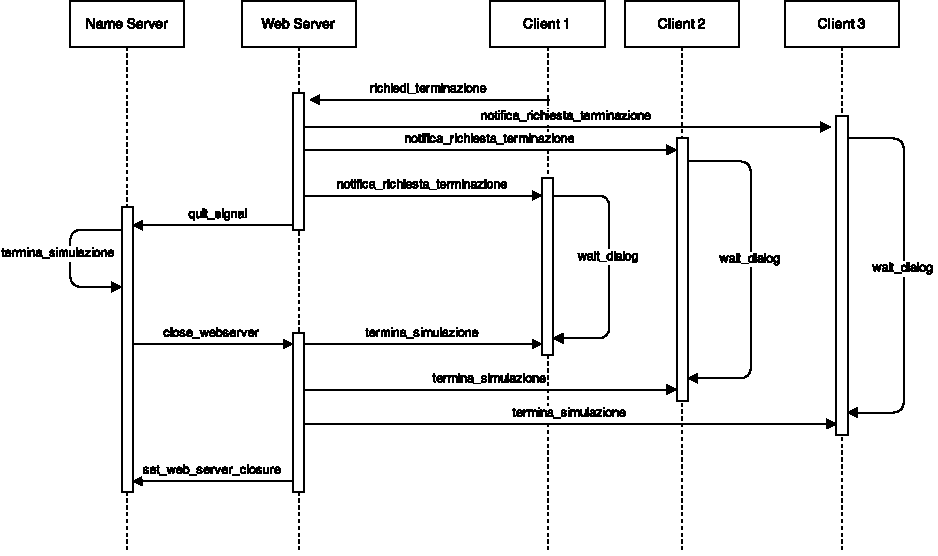
\includegraphics[width=\linewidth]{ChiusuraWebServer}}
\caption{Diagramma di sequenza che descrive la procedura di terminazione della
visualizzazione della simulazione}
\label{fig:stopwebserver}
\end{figure}

\subsection{Client}
Il client ha la possibilità di eseguire tre funzionalità differenti,
implementate ognuna in una pagina web specifica:
\begin{itemize}
	\item visualizzazione della lista dei quartieri attivi
	\item visualizzazione della simulazione di un quartiere
	\item supporto allo sviluppo e preprocessamento dei file di descrizione delle
	mappe
\end{itemize}

\subsubsection{Definizione della mappa}
Il file di definizione della mappa contiene tutte le informazioni necessarie per
eseguire la simulazione di un singolo quartiere. 

L'unità di misura utilizzata nella definizione dei vari elementi è il metro, che
in fase di visualizzazione corrisponderà inizialmente con un pixel sullo
schermo.

All'interno del file di definizione si trovano le descrizioni di:
\begin{itemize}
	\item strade urbane;
	\item strade di ingresso;
	\item incroci con 3 e 4 strade incidenti (descritti separatamente);
	\item luoghi.
\end{itemize}

In aggiunta a quanto elencato sopra, vi si trovano anche informazioni
riguardanti il quartiere e le entità che si muovono in esso (pedoni, bici, auto
e bus).

Di seguito descriveremo le caratteristiche di ogni singola entità.

\paragraph*{Strade urbane}
Le strade urbane sono l'entità principale della definizione della mappa. Sono
caratterizzate da un identificativo numerico e dalla loro posizione all'interno
del quartiere. 

Il sistema di coordinate utilizzato per definire i punti all'interno della mappa
ha l'origine degli assi nell'angolo più in alto a sinistra.

 La posizione della strada è definita da due attributi: \texttt{from} e
 \texttt{to}, ovvero il punto in cui inizia e in cui finisce.
Per questi due valori è stata concordata la seguente convenzione: l'estremo
\texttt{from} è quello avente coordinata x con valore minore. In caso i valori
x dei due estremi siano uguali, l'estremo \texttt{from} è quello avente la y
minore.
Un esempio di questa convenzione è rappresentato in Figura
\ref{fig:polaritastrade}.

\begin{figure}[H] % Example image
\center{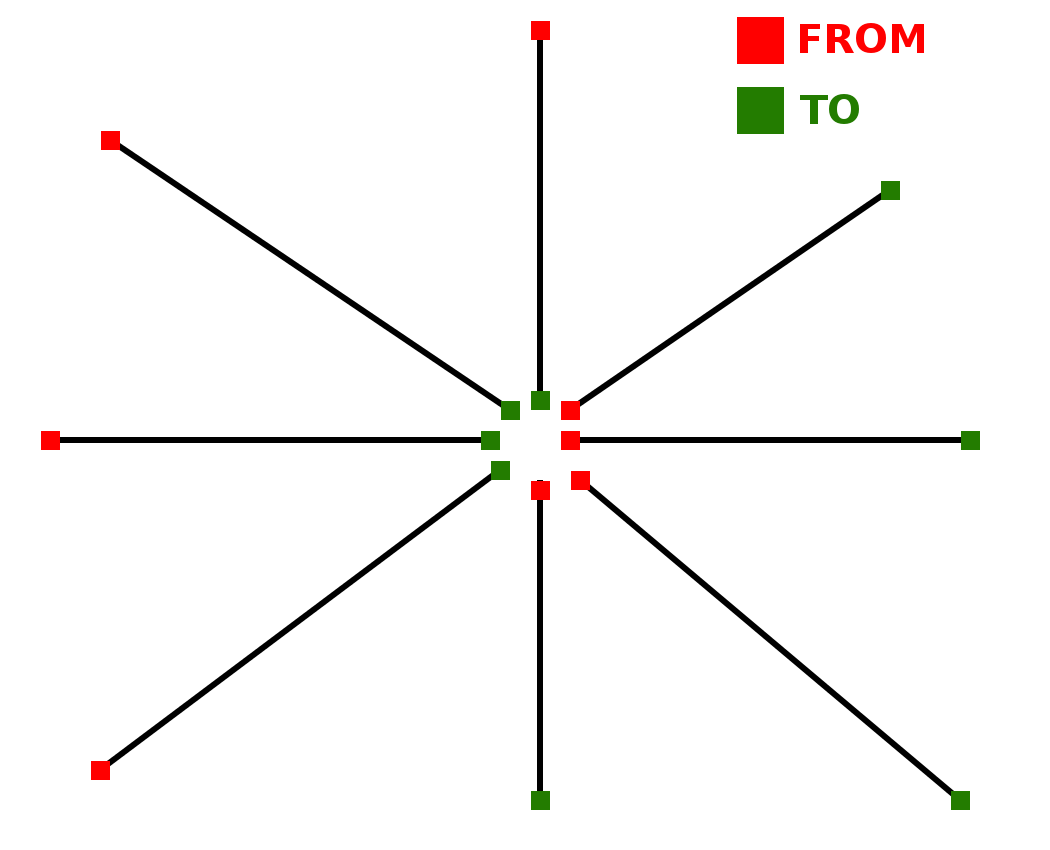
\includegraphics[width=0.8\linewidth]{polarita_strade}}
\caption{Convenzione per la definizione delle coordinate delle strada.}
\label{fig:polaritastrade}
\end{figure}

All'estremo \texttt{from} è associato il valore booleano \texttt{true} mentre
all'estremo \texttt{to} il valore \texttt{false}.
Questa convenzione ci permette di definire in modo univoco come una entità
percorre una strada: le entità viaggiano, da un estremo all'altro di una strada,
utilizzando le corsie o i marciapiedi a destra della linea di mezzaria. Il lato
della strada percorso da una entità è identificato dal valore booleano
dell'estremo verso cui ci si sta dirigendo. Ad esempio, se una macchina si sta
muovendo dall'estremo \texttt{to} all'estremo \texttt{from} allora sta
percorrendo il lato \texttt{true} della strada.

La forma effettiva della strada verrà definita in fase di rendering. Per questo
motivo, la lunghezza effettiva della strada deve essere calcolata processando il
file di descrizione con l'apposita applicazione client.

Ogni strada urbana può definire un numero arbitrario di corsie per senso di
marcia.
Per la realizzazione di questo sistema è stato scelto di fissare questo valore a 2.

\paragraph*{Strade di ingresso}
Le strade di ingresso sono le rappresentazioni dei viali o strade di accesso a
case o edifici. Come le strade urbane, possiedono un identificativo ma sono
prive di estremi \texttt{from} e \texttt{to}.
Per convenzione sono sempre strade prive di curve e sono posizionate in
riferimento ad una strada principale. Per questo motivo, la posizione di queste
strade è definita utilizzando l'id della strada urbana a cui si riferiscono, il
lato della strada dove si immettono e la distanza in metri dall'estremo
\texttt{from}.

Anche questo tipo di strada ammette un parametro che specifica il numero di
corsie per il senso di marcia. Analogamente alle strade urbane, questo è fisso
per la simulazione ed è settato a 1.

\paragraph*{Incroci}
Per motivi di semplicità di realizzazione del sistema di simulazione, si è
distinto tra incroci aventi 4 strade incidenti e incroci aventi 3 strade
incidenti. 

Ogni definizione di incrocio contiene un identificativo e una lista delle strade
incidenti all'incrocio. Per convenzione la prima strada è quella che entra
nell'incrocio da nord, le successive sono quelle che seguono in senso orario.

Gli incroci a tre ingressi presentano un campo addizionale che indica quale
delle strade incidenti non è presente.

Per ogni strada incidente ad un incrocio viene indicato l'identificativo del
quartiere, l'identificativo della strada, il tipo e l'estremo che si affaccia
nell'incrocio.

\paragraph*{Luoghi}
L'ultimo elemento rappresentato nella mappa sono i luoghi. Un luogo può
rappresentare una casa privata, un luogo di lavoro, un qualsiasi edificio o una
fermata per autobus. 

Ogni luogo presenta un identificativo, un nome ed una tipologia. Il
posizionamento viene eseguito utilizzando l'identificativo della relativa strada
di ingresso e delle dimensioni, anch'esse specificate nella definizione del
luogo. Ulteriori dettagli specificano la capienza del luogo in termine di
persone, auto e bici.

\subsubsection{Rappresentazione della mappa}
La rappresentazione grafica della mappa, a partire dalla descrizione di un
quartiere, procede prima caricando tutti gli elementi da visualizzare e poi
disegnandoli effettivamente sullo schermo.

La rappresentazione grafica è realizzata mediante la libreria
Paper.js~\cite{paperjs}, la quale permette di semplificare notevolmente le
operazioni di disegno su di un oggetto Canvas.

Tutte le fasi di caricamento e disegno della mappa vengono eseguite attraverso
uno specifico oggetto JavaScript. Quest'ultimo funge anche da registro per
le strade, incroci e altre entità statiche della mappa.

La prima fase consiste nel creare le istanze degli oggetti strada, incrocio e
lugo, caricarle nei registri e poi collegarle tra loro. La fase di collegamento
è cruciale: le strade di ingresso devono conoscere la posizione della strada
principale a cui sono collegate e gli incroci devono conoscere le strade a loro
incidenti per risolvere la posizione dell'incrocio stesso.

La fase successiva prevede il disegno vero e proprio delle entità sullo schermo.
Le strade incidenti agli incroci, una volta collegate, vengono alterate in modo
da modificarne la forma. Questa operazione permette di inserire curvature che
rendono la strada meno seghettata e più realistica.
Questa fase comprende anche la creazione delle traiettorie utilizzate dalla
simulazione, come descritto nella Sezione \ref{subsec:protocolloavanzamento}.
Tutte le traiettorie vengono indicizzate in modo da essere facilmente reperite
in un secondo momento.

La rappresentazione grafica della mappa non è utilizzata solamente durante la
visualizzazione della simulazione: lo strumento di aiuto allo sviluppo delle
mappe permette di visualizzare la mappa che si sta creando e di calcolare le
lunghezze effettive di strada e traiettorie.
Una volta elaborato con questo strumento, è possibile utilizzare un file di
descrizione di un quartiere nella simulazione effettiva.

\subsubsection{Rappresentazione della simulazione}
La rappresentazione della simulazione utilizza le traiettorie, preparate durante
la fase di rendering della mappa, come delle ``rotaie'' su cui spostare le varie
entità. La posizione di ogni singola entità sulle varie traiettorie è indicata
dai vari aggiornamenti di stato ricevuti dal client.

\paragraph*{Aggiornamenti di stato}
Gli aggiornamenti di stato che arrivano dal sistema di simulazione sono composti
da una lista di entità che si sono mosse durante l'ultimo passo di simulazione. 
Ogni singolo stato è composto dall'identificativo dell'entità ad esso associata,
da un insieme di dati che identifica in modo univoco la traiettoria su cui
l'entità si sta muovendo e la nuova posizione sulla suddetta traiettoria.

\paragraph*{Rendering degli spostamenti per interpolazione}
Lo spostamento effettivo degli oggetti visualizzati dal client procede con una
frequenza di aggiornamento differente rispetto a quella di invio degli stati.
Questa caratteristica richiede l'introduzione di una tecnica di interpolazione.

Utilizzando una tecnica di interpolazione è possibile rappresentare lo
spostamento di un oggetto in maniera fluida, anche quando la frequenza di
aggiornamento dello stato è molto bassa.

Nel caso della nostra simulazione, il tempo che intercorre tra il calcolo di
uno stato e il successivo è pari ad un secondo. Di conseguenza, i client
riceveranno gli aggiornamenti con un intervallo minimo di arrivo pari a un
secondo. Questa frequenza è troppo bassa per permettere una visualizzazione
fluida.

L'interpolazione viene eseguita utilizzando due stati consecutivi.
Indichiamo con $t_{i}^{s}$ e $d_{i}^{s}$ rispettivamente l'istante a cui si
riferisce uno stato e la posizione dell'entità e con $t_{i-1}^{s}$ e
$d_{i-1}^{s}$ istante e posizione dello stato precedente. La durata effettiva
di uno stato ricevuto dal sistema di simulazione sarà quindi:
$$\Delta_{i}^{s}=t_{i}^{s}-t_{i-1}^{s}$$ e sarà pari all'intervallo di
aggiornamento dettato dal sistema di simulazione (pari a un secondo).
Analogamente, lo spostamento effettuato tra i due stati sarà
$$\Delta_{i}^{d}=d_{i}^{s}-d_{i-1}^{s}$$ 
Il sistema di rendering impiega, per ridisegnare la posizione di tutte le
entità, un tempo $$\Delta^{r}<\Delta_{i}^{s}$$ 
Indichiamo con $j$ il numero di operazioni di rendering che possiamo effettuare
nel tempo che intercorre tra l'arrivo di uno stato e il successivo. 
Per semplificare ipotizziamo che questo valore sia intero e che il tempo di
rendering sia costante.
Avremo quindi che $$j=\frac{\Delta_{i}^{s}}{\Delta^{r}}$$
Possiamo ora aumentare la frequenza di aggiornamento interpolando ogni
$\Delta^{r}$ la posizione effettiva dell'entità.
Calcoliamo quindi la posizione effettiva con la seguente formula:
$$d_{k}^{e}=d_{i-1}{s}+k\cdot\frac{\Delta_{i}^{d}}{j}$$ al $k-esimo$ passo di
rendering tra gli stati $i-1$ e $i$, con $0 \leq k \leq j$.

Possiamo calcolare la posizione effettiva delle varie entità con una frequenza
inferiore a quella di arrivo degli stati utilizzando come stato di base il
penultimo ricevuto e adottando la tecnica dell'interpolazione.

Le semplificazioni fatte durante la dimostrazione della tecnica non sono state
adottate nell'implementazione, la quale gestisce tempi di rendering non
costanti.

Utilizzando questa tecnica si nota subito che la simulazione sarà visualizzata
dall'utente con un ritardo minimo pari alla durata di uno stato.

\paragraph*{Gestione degli stati}
Per garantire una visualizzazione fluida e continua è stata adottata una tecnica
di buffering degli stati. A causa delle caratteristiche di rete, il tempo che
intercorre tra la ricezione di uno stato e il successivo può non è costante. Nel
caso in cui questo tempo superi quello prestabilito dal sistema la
visualizzazione della simulazione subisce un arresto.

Per evitare questo fenomeno è stato introdotto un buffer che salva un numero di
stati prima di cominciare la visualizzazione. In questo modo è possibile fare
affidamento ad una scorta di stati qualora la ricezione subisca un
rallentamento.

Per evitare un inutile spreco di risorse, molti browser evitano di ridisegnare
la pagina quando essa non è attiva. Questa caratteristica induce nel nostro
sistema un accumulo di stati ed una pausa nella simulazione. Per ovviare a
questo problema è stata implementata una funzionalità che permette, quando
l'utente riattiva la finestra del browser, di scartare tutti gli stati ricevuti
tranne i più recenti. In questo modo l'utente visualizzerà sempre e solo lo
stato corrente del sistema.

\section{Tecnologie utilizzate}
Le tecnologie utilizzate per lo sviluppo del prototipo sono state scelte valutando principalmente il modello di concorrenza offerto dal linguaggio. Quindi è stato scelto ADA dato che il modello di concorrenza che il linguaggio offre si presta in modo tale da distinguere in modo chiaro le entità protagoniste in una realtà concorrente: task, risorse, code di attesa, ecc. Per quanto riguarda la distribuzione è stato sfruttato sempre il modello di distribuzione di ADA, ovvero ADA DSA, e quindi il middleware di PolyORB. \\
Ogni partizione del sistema è stata sviluppata quindi in ADA; la scelta di utilizzare DSA limita la portabilità dell'applicazione, ma è stato scelto comunque a discapito della portabilità, valutando principalmente la trasparenza con cui DSA permette di realizzare un sistema distribuito, e quindi la quantità di lavoro richiesto per implementare il prototipo.
%\newpage
\pagebreak
\listoffixmes

\appendix


\bibliographystyle{abbrvnat}
\bibliography{bibliografia}
\end{document}

